%!TEX program = luatex

\documentclass[12pt]{article}
\usepackage[margin=1in]{geometry}
\usepackage{fontawesome}
\usepackage{fontspec}
\usepackage[hidelinks]{hyperref}
\usepackage{pdfpages}
\usepackage{csquotes}
\MakeOuterQuote{"}
\setmainfont{Palatino Linotype}
\setsansfont{Myriad Pro}
\setmonofont{Andale Mono}
\usepackage{microtype}
\usepackage{color}
\usepackage{lettrine}
\usepackage{changepage}
\usepackage{wrapfig}
\usepackage{xfrac}

\setlength{\parindent}{1em}
\setlength{\parskip}{12pt}

\definecolor{fsuMaroon}{RGB}{155,0,33}

\newcommand{\dueDate}[1]{\textbf{\textcolor{fsuMaroon}{#1}}}

\begin{document}

\begin{center}
\noindent\large\dueDate{\faBriefcase}~~\textsf{\textit{Project Package:} Argument Essay}\normalsize\\
\rule{4in}{1pt}
\end{center}

This essay project helps you in two ways. First, it helps you develop a \emph{mindset} and \emph{approach} to technology in teaching and learning. Second, if you need to take the Praxis Core Academic Skills for Educators Exam, this will help prepare you to succeed on the Argument writing part of the test. \textbf{Here is your writing prompt:}

\begin{adjustwidth*}{4em}{2em}
\noindent\blockquote[Marc Prensky, "Teaching Digital Natives"]{\ldots[T]he digital technology now coming,  more or less rapidly, into our classrooms\textemdash{}if used properly\textemdash{}can help make our students’ learning real, engaging, and useful for their future.}
\end{adjustwidth*}

\begin{wrapfigure}{R}{0.20\linewidth}
	
\includegraphics[width=\linewidth]{graphics/computer-classroom.png}
\end{wrapfigure}


Your job is to construct an argument \emph{in support of} Marc Prensky’s statement about technology’s place in education (Prensky, 2010). Remember that\textemdash{}as Grant Wiggins (2015) points out\textemdash{}arguments are written to \emph{demonstrate your understanding} of a topic so that your reader will consider your ideas when forming their own position rather than persuading your reader that you are right.

Your argument should be single-spaced, between 1 \textbf{full} page and 2 pages long. Remember to use the \emph{argument structure:} (1) introduction that highlights the importance of the topic, (2) your \textit{claim} and at least two items of \textit{evidence} you bring to support your claim, (3) \textit{reasoning} that connects your evidence to your claim and helps your reader better understand your evidence, and (4) your conclusion that summarizes your argument. You are highly encouraged to draw on your own experiences, things that you have read outside of class, and the readings you have completed for this class. This next part is different than the requirements of the Core Exam, but if you do quote or refer to a reading, make sure to use APA format for in-text citations (see the \textit{Course Tools and Practices} document for more information). Include a list of references at the end of your essay.

Here are some resources to help you successfully complete this essay:
\begin{itemize}
	\itemsep-0.5em
	\item \emph{\textbf{The readings for class so far}}
	\item Praxis Core Writing Exam Study Companion (\url{https://www.ets.org/s/praxis/pdf/5722.pdf})
	\item Video about hyperbole (\url{http://goo.gl/MUtnU4})
	\item The \textit{Course Tools and Practices} Document
\end{itemize}

\vfill

\begin{center}\rule{4in}{1pt}\end{center}
\noindent\lettrine{\dueDate{\faCalendar}}{~~}\normalsize\textsf{You should plan on visiting the Writing Center with a draft of your essay and 2-3 questions by \dueDate{September~11}. The final draft of your essay is due in \texttt{TaskStream} by \dueDate{September~18}. Schedule a meeting with your professor to discuss your feedback by \dueDate{October 16}.}

\newpage

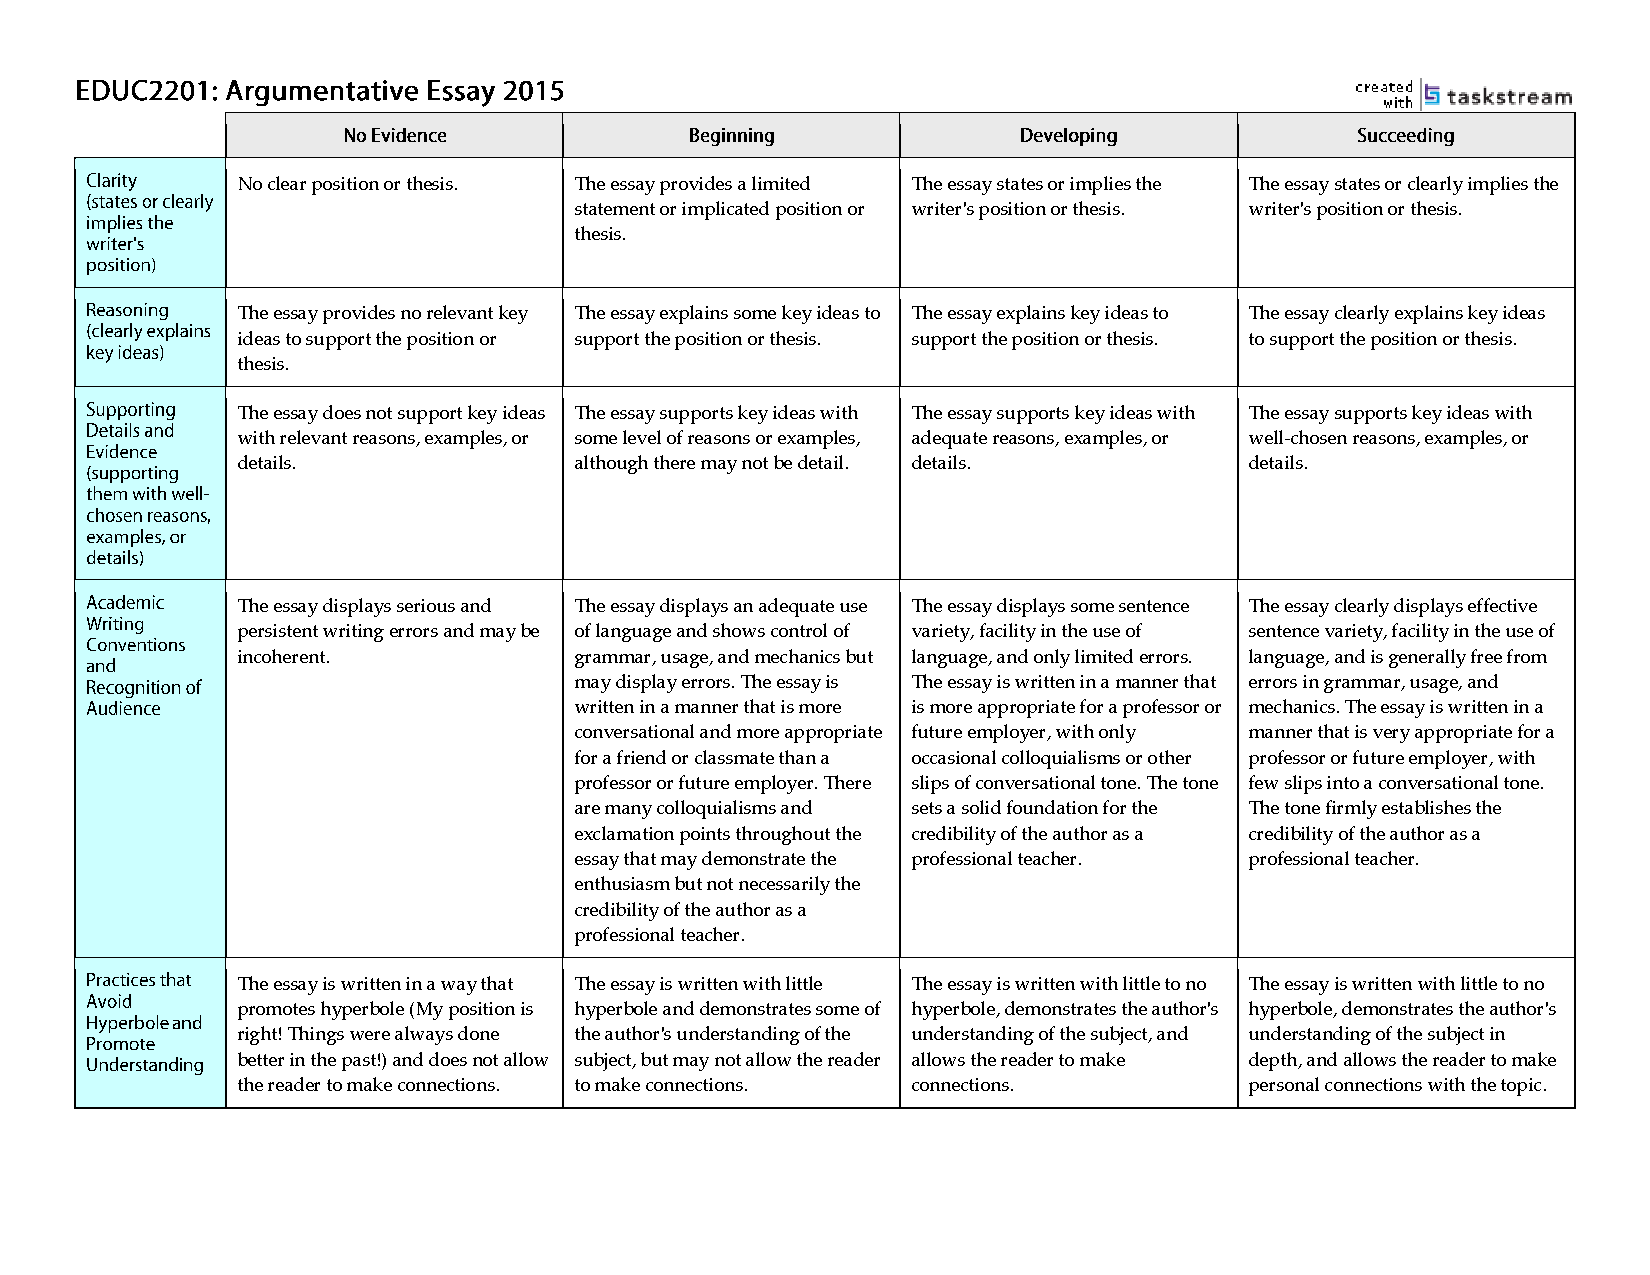
\includepdf[angle=90,width=8in]{educ2201-rubric-argument.pdf}

\end{document}
